\label{Bijlage 1}

\appendix
\section{Bijlage 1: Versie Systeembeheer GIT}

\subsection*{Installatie en gebruik}\ \\[12pt]

Voor het gebruiken van Git bash gebruiken we msygit. Na de installatie van het programma gebruiken we de "Git Bash" en gebruiken we volgende twee commando's om ons te kunne identificeren. Dit zal later zijn nut bewijzen.\\
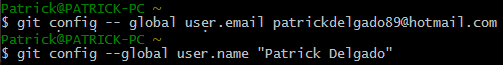
\includegraphics[width=0.7\textwidth]{git1.png}\\


Als volgende moet er een SSH Key gegenereerd worden. Deze zal zorgen voor de connectie tussen de documenten op de pc van de gebruiker en de online repository.\\

Voor het maken van deze sleutel worden volgende commando gedaan.\\
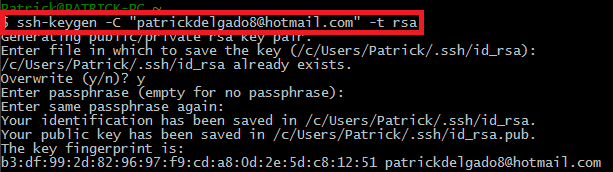
\includegraphics[width=0.7\textwidth]{git2.png}\\

Dit zal een folder .ssh aanmaken in de User directory met de bestanden (id-rsa en id-rsa.pub). Het .pub bestand zullen we later nodig hebben voor de online repository server later.\\

In de windows explorer rechter muisklikken we op de map die we willen linken aan de online repository en kiezen we "Git Bash Here". Dit zal de Git Bash rechtstreeks openen met de link naar deze map en geven we het commando "git init" in. Dit zal de map in een git repository omvormen. In de map zelf wordt ook de map .git aangemaakt (normaal als verborgen), als deze verwijderd wordt zal de hoofdmap niet langer als een Git repository gezien worden.\\

Met het commando "git status" krijgen we een lijst van alle nieuwe, aangepaste of verwijderde bestanden te zien die nog niet doorgevoerd zijn naar de online repository (deze is momenteel nog niet aangemaakt maar hier wordt later op terug gekomen).\\
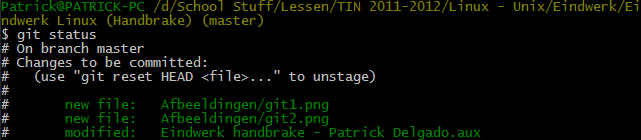
\includegraphics[width=0.7\textwidth]{git3.png}\\

Om de volledige map met al zijn bestanden voor te bereiden voor verplaatsing naar de online repository doen we het commando "Git add .".\\
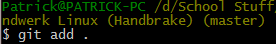
\includegraphics[width=0.7\textwidth]{git4.png}\\

Als nu het commando "git status" gedaan wordt toon een lijst met alle veranderingen die zullen gebeuren. Hierna wordt het commando "git commit -m <bericht>" gedaan om deze veranderingen klaar te zetten voor door te sturen . Dit is een soort van toestemming geven aan het systeem om later deze wijzigingen door te voeren.\\
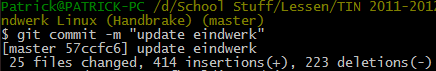
\includegraphics[width=0.7\textwidth]{git5.png}\\

Om verder te kunnen moeten we ons een repository maken. Op de site "www.github.com" kan men zich registeren voor een gratis account en opslagruimte. Na het aanmaken van een account moet de SSH key toegevoegd worden om de link te kunnen leggen van online opslag naar computer. Hiervoor gebruiken we het id-rsa.pub bestand. Open deze met notepad en kopieer de volledige inhoud. Bij de account instellingen is een gedeelte "SSH-Key" en deze voegen we hier toe.\\

Nu is het tijd om een repository te maken. Dit wordt gewoon gedaan op de Github hoofdpagina van de gebruiker via de knop "New repository". Verder hebben we volgende link nodig om verder te kunnen.\\

\includegraphics[width=0.7\textwidth]{git6.png}\\

Terug in de Git Bash gebruiken we volgend commando om de repository nu volledig te linken aan ons systeem.\\
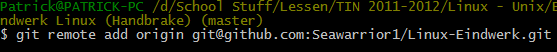
\includegraphics[width=0.7\textwidth]{git7.png}\\

Nu kunnen de bestanden naar de repository upgeload worden met het commando "git push origin master". Alle bestanden die in de eerdere commit stonden worden nu ge pushed naar de server voor online opslag.\\
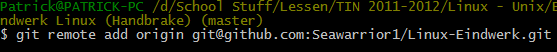
\includegraphics[width=0.7\textwidth]{git7.png}\\

Verder commano



